\section{Experiment 1: Rotated Bars}
\label{section:rotatedLines}
\subsection{Introduction}
The goal of this task was to recreate example 2 from \citet{nessler}. In this example they fed a winner-take-all spiking neural network images with bars in different orientations on them. The network then clustered the images into ten groups depending on their orientation.

\subsection{Methods}
\paragraph{Input data}
The images used in this task were generated with a size of 29 x 29 pixels. Black bars with a width of 7 pixels going through the center of the image were drawn onto a white background. To simulate noise each pixel had a chance of ten percent to have its color flipped. To ensure that all bars in the images have the same length regardless of their orientation a circular mask with a radius of 15 pixels was applied to the images. This recolored all pixels outside of the mask to white. During the training of the network one image per iteration was generated in a uniformly distributed orientation and each image was shown for 200 ms. For the training of the network 4000 of these images were shown. The randomly chosen orientation could lie between 0 and 359 degrees.  Two examples of such images can be seen in Figure \ref{fig:angleImages}.

\begin{figure}
  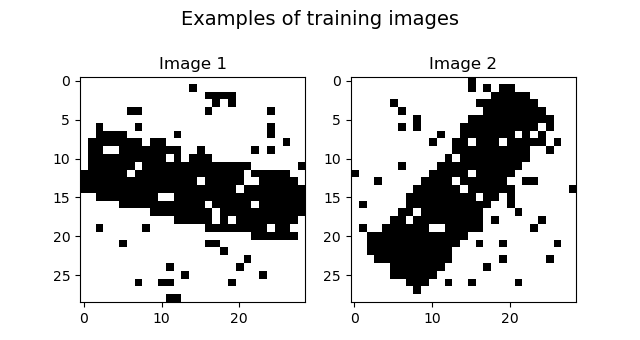
\includegraphics[width=\linewidth]{figures/angleNetwork/trainingImages.png}
  \caption{Two examples of the generated training data in this experiment.}
  \label{fig:angleImages}
\end{figure}

\paragraph{Neuron model}

As in \citet{nessler} the input neurons X are firing according to a poisson process with an average firing rate of 20 Hz when active and with 0 Hz when in an inactive state. The excitatory post synaptic potentials (EPSPs) $x_i(t)$ that these neurons produce can be seen in Figure \ref{fig:XSpike}. A double exponential kernel was used to generate the EPSP. The time constant for the rise of the signal $\tau_{rise}$ was 1 ms and the time constant for the decay of the signal $\tau_{decay}$ was 15 ms. The addition of the time step size $\delta t$ was necessary to get the time t at the end of the current simulation step. $t_f$ is the time at which the spike of $x_i$ occurred
\begin{equation}
\label{eqn:EPSP}
x_i(t) = e^{-(t + \delta t - t_f) / \tau_{decay}} - e^{-(t + \delta t - t_f) / \tau_{rise}}.
\end{equation}


\begin{figure}
  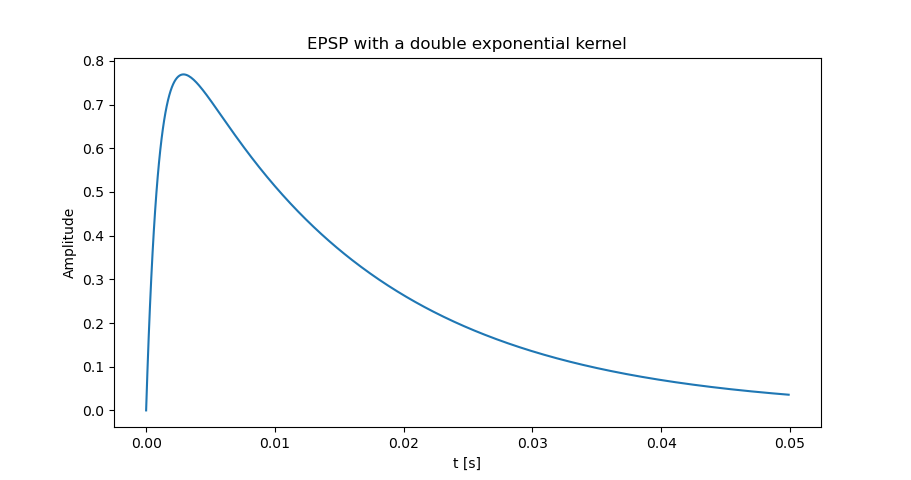
\includegraphics[width=\linewidth]{figures/XSpike.png}
  \caption{Form of an excitatory post synaptic potential generated by an input neuron over time. A double exponential kernel was used to generate this signal. These signals are fed to the next layer of the network. }
  \label{fig:XSpike}
\end{figure}

The firing rate of an output neuron $y_k$ is given by
\begin{equation}
\label{eqn:rk}
r_k(t) = e^{u_k(t) - I(t)}.
\end{equation}
The probability of an individual output neuron to fire within a time step $\delta t$ is given by
\begin{equation}
\label{eqn:rkdt}
r_k(t) \cdot \delta t.
\end{equation}

\paragraph{Network architecture}
Each pixel of an input image was connected to two neurons. The first of these neurons is in an active state when the pixel is black and in an inactive state otherwise. The second neuron expresses the opposite behaviour. As a consequence the network needs 1682 ($29 \cdot 29 \cdot 2$) excitatory input neurons $x_1,...,x_n$. These input neurons are fully connected to ten excitatory output neurons $y_1,...,y_k$. This means that that every input neuron $x_i$ is connected to each output neuron $y_k$. The membrane potential $u_k$ of each output neuron is calculated by multiplying the EPSP of each input neuron times the weight of the connection between them
\begin{equation}
\label{eqn:uk}
u_k(t) = \sum_{i=1}^n w_{ki} \cdot x_i(t).
\end{equation}
In \citet{nessler} each output neuron $y_k$ also had an intrinsic excitability $w_{k0}$ which was learned for each neuron. For this experiment however it was omitted, as each orientation of input images was equally likely, thus the intrinsic excitability of each output neuron would end up being the same.

The output neurons are modelled in a winner-takes-all (WTA) circuit. This means that whenever one output neuron spikes, a lateral inhibitory signal is fed to all output neurons, thus preventing the further activation of them for $\sigma_{inh} = 5 ms$. After completion of the training of the network each output neuron should be active for bars in a coherent area. Each of those areas should ideally be of equal size. As the bars can be oriented between 0 and 359 degrees, but each 180 degree rotation of an image results in an equivalent image, the desired size of the active area of an output neuron should be 18 degrees.


\paragraph{Inhibition}
The inhibition signal was chosen to depend on the current membrane potential of the output neurons. According to \citet{nessler} the total firing rate of the output neurons is
\begin{equation}
\label{eqn:R}
R(t) = \sum_{k=1}^K e^{u_k(t) - I(t)}.
\end{equation}
Solving this equation for I(t) yields
\begin{equation}
\label{}
R(t) = \frac{ \sum_{k=1}^K e^{u_k(t)}}{e^{I(t)}}
\end{equation}
\begin{equation}
\label{}
e^{I(t)} = \frac{\sum_{k=1}^K e^{u_k(t)}}{R(t)}
\end{equation}
\begin{equation}
\label{}
I(t) = \ln{ \frac{ \sum_{k=1}^K e^{u_k(t)}}{R(t)}}
\end{equation}
\begin{equation}
\label{eqn:I(t)}
I(t) =  - \ln{R(t)} + \ln{  \sum_{k=1}^K e^{u_k(t)}}.
\end{equation}
When implementing the inhibition the $- \ln{R(t)}$ term of Equation \ref{eqn:I(t)} was overlooked, that means it was assumed to be zero. Because of that R(t) equals 1 when the inhibition is active. This error was not detected at first, as the chance that a Y neuron fires within a time step of 1 ms with active inhibition is 1/1000 due to that oversight.

Whenever an output neuron produces a spike the inhibition signal I(t) is subtracted from the membrane potential $u_k(t)$ of every output neuron. This happens for the duration of $\sigma_{inh} = 5 ms$. Thus follows

\begin{equation}
\label{eqn:iinh}
I(t) = \begin{dcases*} \ln ( \sum_{i=1}^k e^{u_k} ) & if any $y_k$ fired in $ [t^f, t^f  + \sigma_{inh}] $ \\
0 & \text{if any $y_k$ did not fire in $ [t^f, t^f + \sigma_{inh}] $. } \end{dcases*}\end{equation}

\paragraph{Spike timing dependent plasticity}
The weights $w_{ki}$ between neurons $x_i$ and $y_k$ are updated whenever an output neuron fires. The time window $\sigma$ was set to 10 ms according to \citet{nessler}. If $y_k$ produces a spike all its weights are updated as
\begin{equation}
\label{deltawki}
\Delta w_{ki} = \begin{dcases*} \lambda \cdot (ce^{-w_{ki}} - 1) & if $x_{i}$ fired in $ [t^f - \sigma, t^f] $ \\
\lambda \cdot (-1) & \text{if $ x_i $ did not fire in $ [t^f - \sigma, t^f] $, } \end{dcases*}
\end{equation}
where $\lambda$ is the learning rate, the parameter c shifts the weight values, $t^f$ is the time when $y_k$ spiked and $\sigma$ is the time window in which input spikes are considered as "before" an output spike. As the membrane potentials $u_k$ of the output neurons result from the addition of the EPSPs of the 1682 input neurons times the corresponding weight, a way to control the average size of u is needed. If u is to small the output neurons will fire too sparsely and if u is too big it will impair the learning process. So to limit u, the size of the weights is controlled via the parameter c. The learning rate $\lambda$ is needed to control the size of each weight update. If it is too big few output neurons will take over more than the expected 18° areas and others will only respond for smaller areas or not at all. On the other hand if $\lambda$ is too small the network will learn very slowly and may never converge. Due to these two parameters being unwieldy to determine analytically they were chosen via grid search. 


\subsection{Results}

\paragraph{Parameter search}
The two parameters c, which controls the size of the weights, and the learning rate $\lambda$ were fitted to the network via grid search.	The tested parameters were as follows:
\begin{itemize}
  \item $c = 1$ ($\lambda = 10^{-2}, 10^{-3}, 10^{-4}$) 
  \item $c = 10$ ($\lambda = 10^{-2}, 10^{-3}, 10^{-4}$) 
  \item $c = 20$ ($\lambda = 10^{-2}, 10^{-2.5}, 10^{-3}, 10^{-3.5},  10^{-4}, 10^{-4.5}, 10^{-5}$) 
  \item $c = 30$ ($\lambda = 10^{-2}, 10^{-2.5}, 10^{-3}, 10^{-3.5}$) 
\end{itemize}
The simulation was conducted by simulating small discrete time steps and calculating the changes of the network in each step. The step size $\delta t$ was chosen as 1 ms.

\paragraph{$c = 1$}
The best results for $c = 1$ were achieved with $\lambda = 10^{-2}$. But overall this value for c did not work, even tough the network did learn to cluster images into eight groups depending on their orientation. In Figure \ref{fig:c1Pie} one can see which output neuron was the most active during the training process for each angle in 1° steps.

\begin{figure}
  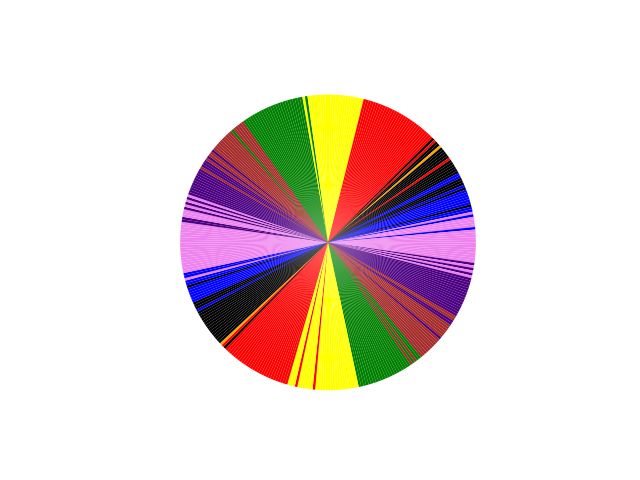
\includegraphics[width=\linewidth]{figures/angleNetwork/c1Pie.png}
  \caption{Most active output neuron depending on orientation of the training image during the training process. $c = 1, \lambda = 10^{-2}$}
  \label{fig:c1Pie}
\end{figure}

In Figure \ref{fig:c1Distinct} the training progress of the network can be seen. The figure shows the number of distinct output neurons active during the presentation of each training image shown. Due to the large learning rate, compared to other values of c,  the network learned quickly. However after iteration 70 there were images shown for which not a single output neuron spiked. This dying out of the networks activity is due to the parameter c being too small, which leads to too low membrane potentials.

\begin{figure}
  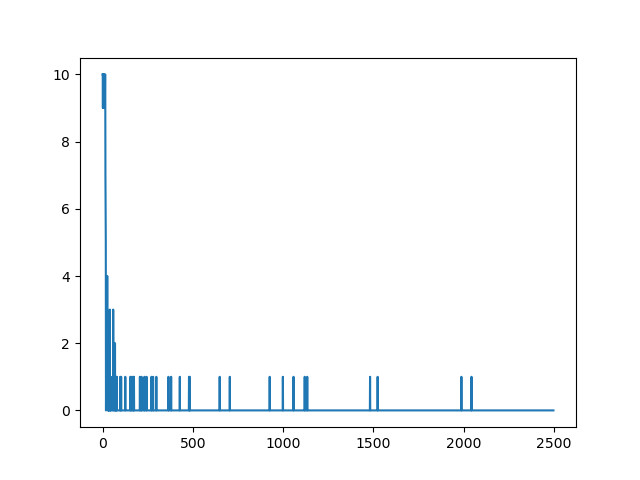
\includegraphics[width=\linewidth]{figures/angleNetwork/c1Distinct.png}
  \caption{Number of distinct output neurons active during the presentation duration of each training image. x-axis: image shown, y-axis: distinct output neurons active, $c = 1, \lambda = 10^{-2}$}
  \label{fig:c1Distinct}
\end{figure}

\paragraph{$c = 10$}
This value of $c = 10$ had the same problem of the network activity dying out as $c = 1$ although at a later point in time, as can be seen in Figure \ref{fig:c10Distinct}. Also in Figure \ref{fig:c10LastSpikes} the last 50 output spikes of the training process can be seen. As indicated by Figure \ref{fig:c10Distinct} the activity is sparse.

\begin{figure}
  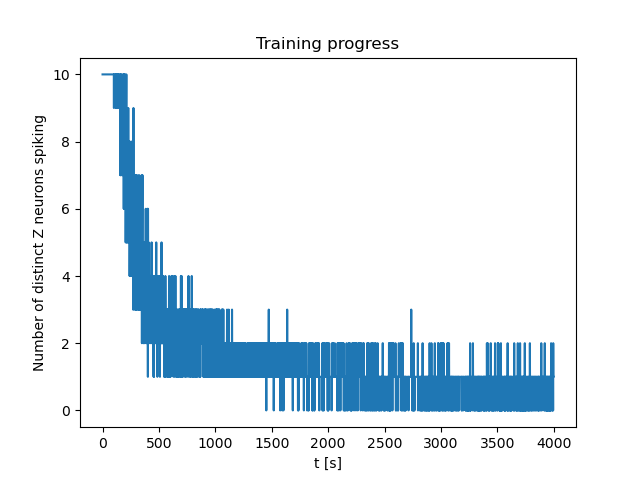
\includegraphics[width=\linewidth]{figures/angleNetwork/c10_3distinctZ.png}
  \caption{Number of distinct output neurons active during the presentation duration of each training image. x-axis: image shown, y-axis: distinct output neurons active, $c = 10, \lambda = 10^{-3}$}
  \label{fig:c10Distinct}
\end{figure}

\begin{figure}
  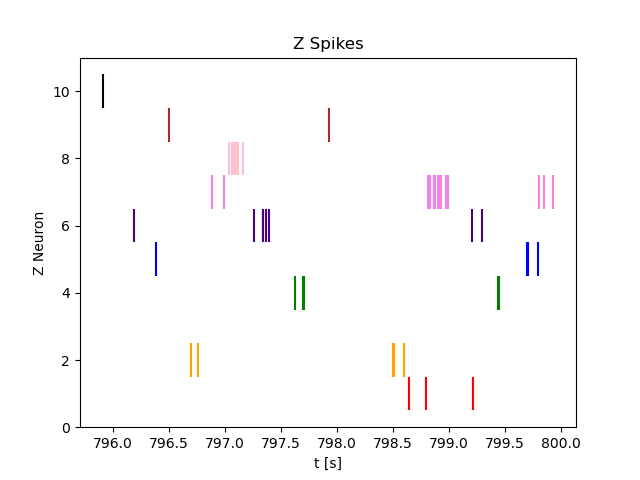
\includegraphics[width=\linewidth]{figures/angleNetwork/c10_3_50LastZSpikes.png}
  \caption{Last 50 output neuron spikes, $c = 10, \lambda = 10^{-3}$}
  \label{fig:c10LastSpikes}
\end{figure}

\paragraph{$c = 20$}
$c = 20$ was the first value for which the network activity did not die out after some time. For $\lambda = 10^{-2}$ one output neuron learned to spike first for every possible input image orientation, see Figure \ref{fig:c20_2Pie}. 

\begin{figure}
  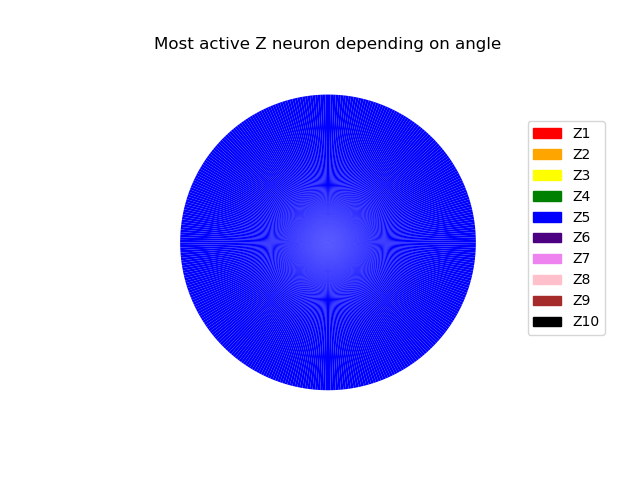
\includegraphics[width=\linewidth]{figures/angleNetwork/c20_2pie.png}
  \caption{Most active output neuron depending on orientation of the training image during the training process. $c = 20, \lambda = 10^{-2}$}
  \label{fig:c20_2Pie}
\end{figure}

With $c = 20$ and $\lambda = 10^{-3}$ the first combination that yielded a stable network was found. In Figure \ref{fig:c20_3Distinct} the amount of distinct output neurons firing during the presentation of each training image can be seen. Figure \ref{fig:c20_3averageZ} shows the proportion of the most active output neuron to all other output neurons active for each training image. Both of these figures can be used to measure the training progress of the network. Figure \ref{fig:c20_3averageZ} however shows the additional information how certain the network is that a training image belongs to a specific group.

\begin{figure}
  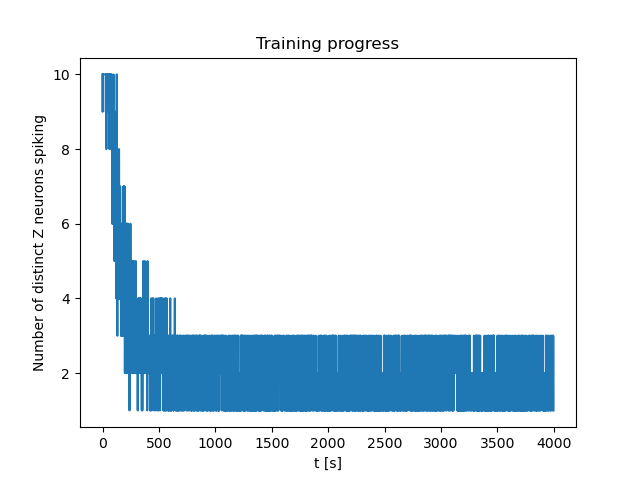
\includegraphics[width=\linewidth]{figures/angleNetwork/c20_3distinctZ.png}
  \caption{Number of distinct output neurons active during the presentation duration of each training image. x-axis: image shown, y-axis: distinct output neuron active, $c = 20, \lambda = 10^{-3}$}
  \label{fig:c20_3Distinct}
\end{figure}

\begin{figure}
  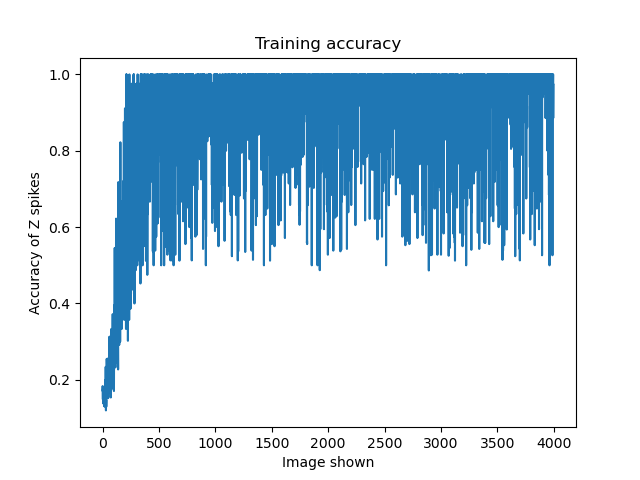
\includegraphics[width=\linewidth]{figures/angleNetwork/c20_3averageZ.png}
  \caption{Proportion (accuracy) of most active output neuron  to activity of all other output neurons during the presentation duration of each training image. $c = 20, \lambda = 10^{-3}$}
  \label{fig:c20_3averageZ}
\end{figure}

As this network did not die out after some time the trained network was analysed further. 180 images were generated in 1° steps and each was shown to the network for 200 ms. During each image presentation duration the most active output neuron was recorded. This yielded Figure \ref{fig:c20_3Pie}.

\begin{figure}
  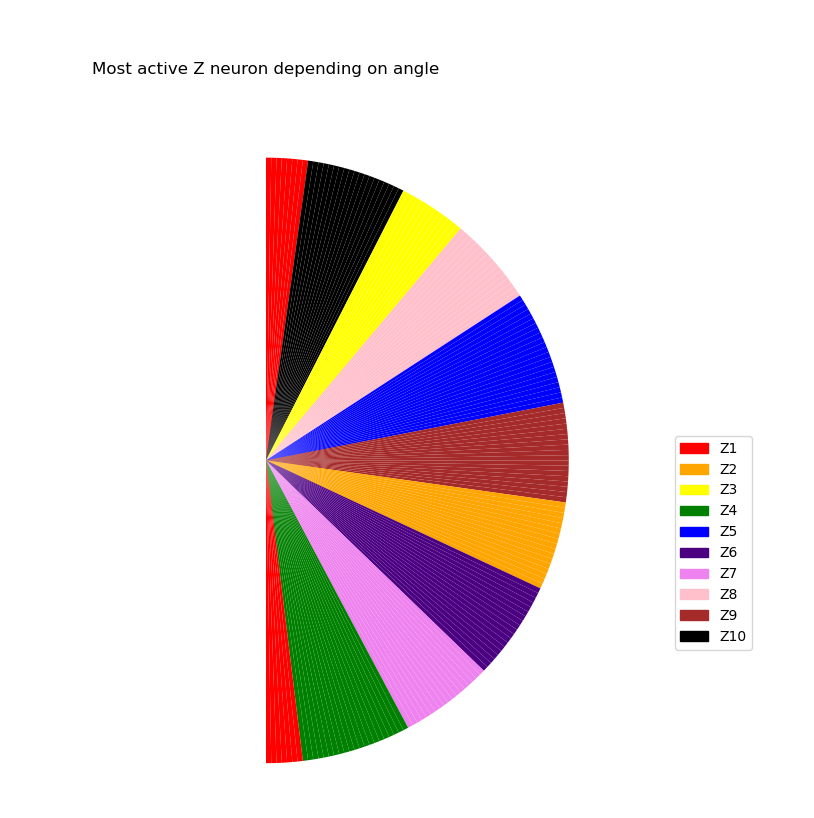
\includegraphics[width=\linewidth]{figures/angleNetwork/c20_3validationPie.png}
  \caption{Most active output neuron depending on orientation of the training image during the training process. $c = 20, \lambda = 10^{-3}$}
  \label{fig:c20_3Pie}
\end{figure}

Also the number of distinct output neurons firing during each image presentation was recorded and is shown in \ref{fig:c20_3validationDistinctZSpikes}. In this figure it seems that the points in which there are three distinct output neurons active are periodic in nature. This can be explained by Figure \ref{fig:c20_3validationZSpikes}. There it can be seen that whenever the image orientation nears the border between two competing output neurons both start to be active. This explains why for large parts of Figure \ref{fig:c20_3validationDistinctZSpikes} 2 neurons are active, as large portions of the bar in the image is overlapping the areas of the two nearest output neurons, thus producing high membrane potentials for both. The third distinct output neuron that is occasionally active seems to be of stochastic nature as much of the bars in the images overlaps areas of all other output neurons, thus generating a non zero membrane potential for each output neuron. However the occurrence of 3 distinct active output neurons seems to mostly occur at or close to the border between two competing output neurons, as there are already 2 distinct neurons firing by design.

\begin{figure}
  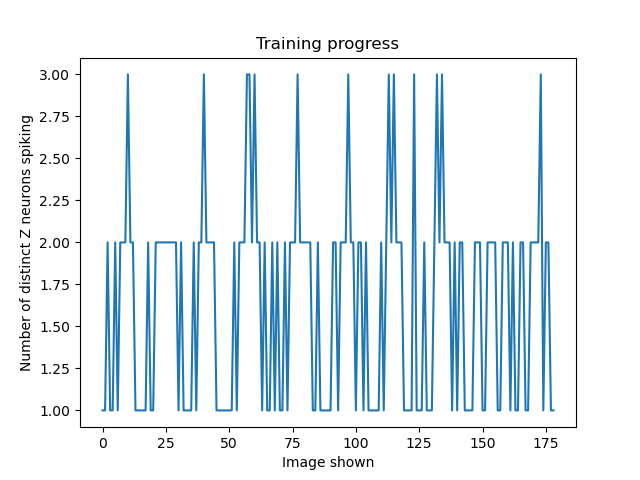
\includegraphics[width=\linewidth]{figures/angleNetwork/c20_3validationDistinctZSpikes.png}
  \caption{Number of distinct output neurons active during the presentation duration of each training image. x-axis: image shown, y-axis: distinct output neuron active, $c = 20, \lambda = 10^{-3}$}
  \label{fig:c20_3validationDistinctZSpikes}
\end{figure}

\begin{figure}
  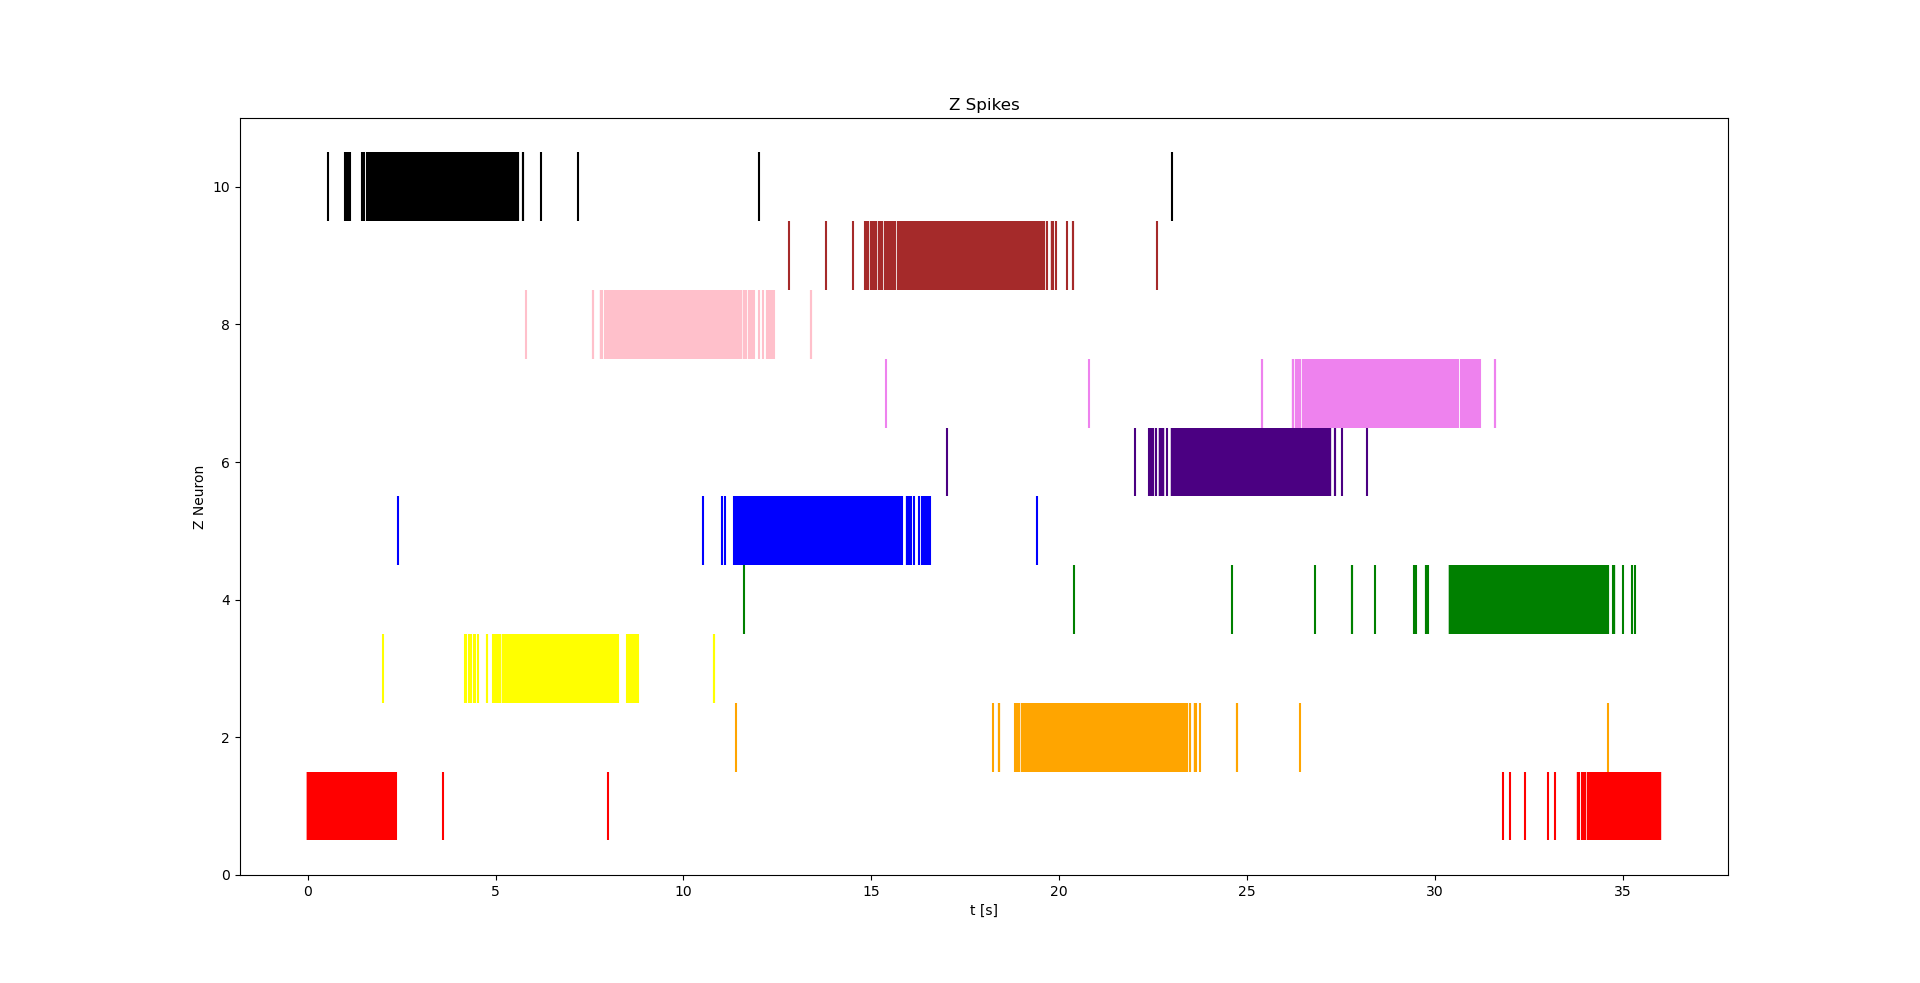
\includegraphics[width=\linewidth]{figures/angleNetwork/c20_3validationZSpikes.png}
  \caption{Output spikes over the presentation of input images from 0 to 179°, $c = 20, \lambda = 10^{-3}$}
  \label{fig:c20_3validationZSpikes}
\end{figure}

Also it was possible to project the learned weights $w_{ki}$ into the 2-D space to observe what they represent. This projection can be seen in Figure \ref{fig:c20_3weights2.png} for the weights of $y_{10}$.

\begin{figure}
  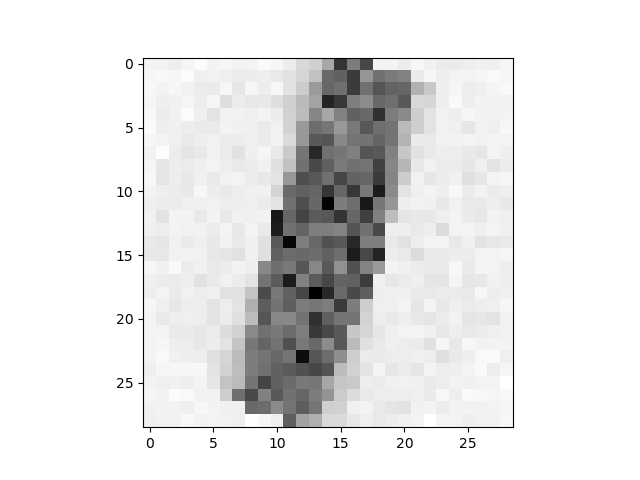
\includegraphics[width=\linewidth]{figures/angleNetwork/c20_3weights2.png}
  \caption{Visualization of the learned weights of $y_{10}$.}
  \label{fig:c20_3weights2.png}
\end{figure}

The results for smaller $\lambda$ were also valid, but they did not seem to yield superior results to the parameters $c = 20$ and $\lambda = 10^{-3}$. As with smaller learning rates the training simply took longer and the performance of the network did not improve they were discarded and  the learning rate $\lambda = 10^{-3}$ was declared winner for $c = 20$. To save space the figures of smaller learning rates will not be shown here.

\paragraph{$c = 30$}
also yielded a functioning network, but it did perform analogous to $c = 20$. It did perform in the same way, as with $c = 20$ the output neurons already fire every 5 ms, slowed down by the inhibition. By increasing c further the output neurons did not increase their activity.

\subsection{Conclusion}

The parameters $c = 20$ and $\lambda = 10^{-3} $ were finally chosen as the network performed the best and trained the quickest with these parameters, without raising the membrane potential needlessly.







\section{Experiment 3: Rotated bars with adaptive inhibition}
\label{section:rotatedLinesAdaptiveInhibition}

\subsection{Introduction}

This experiment analyses a different approach to the implementation of the inhibition of the output neurons. 
In Experiment \ref{section:rotatedLines} and \ref{section:horvert} the output neurons were stopped from firing for a defined time window after any output neuron fired. The time window during which the inhibition was active was 5 ms, which resulted in an average output firing rate of 200 Hz. In this experiment an adaptive inhibition will be used which will regulate the membrane potentials of the output neurons so that all of them together fire with 200 Hz on average. The distinction to the previous experiments is that there never is a time window in which no output neuron may fire. Also it is assumed that the weight shifting parameter c will not be needed to be fitted to the network, as the adaptive inhibition regulates the output firing rate of the network.

\subsection{Methods}

The adaptive inhibition is given by Equation \ref{eqn:I(t)} which was already used in Experiments \ref{section:rotatedLines} and \ref{section:horvert}. However the total output firing rate $R(t)$ was set to 200 Hz in this experiment.

\subsection{Results}

Several different values for the parameter c were tested. As expected the firing rate of the output neurons 200 Hz on average regardless of the value of c. However for values of c bigger than 100 the network did not learn correctly. For those values some output neurons learned to respond to areas of more than 18°, while other neurons did not respond to any areas. For $c = 20$ the network performed equally to Experiment \ref{section:rotatedLines}. The results for that parameter can be seen in Figures \ref{fig:angleNetworkAdaptiveInhibitionTraining}, \ref{fig:angleNetworkAdaptiveInhibitionOutputFiringRate} and \ref{fig:angleNetworkAdaptiveInhibitionValidation}.


\begin{figure}
  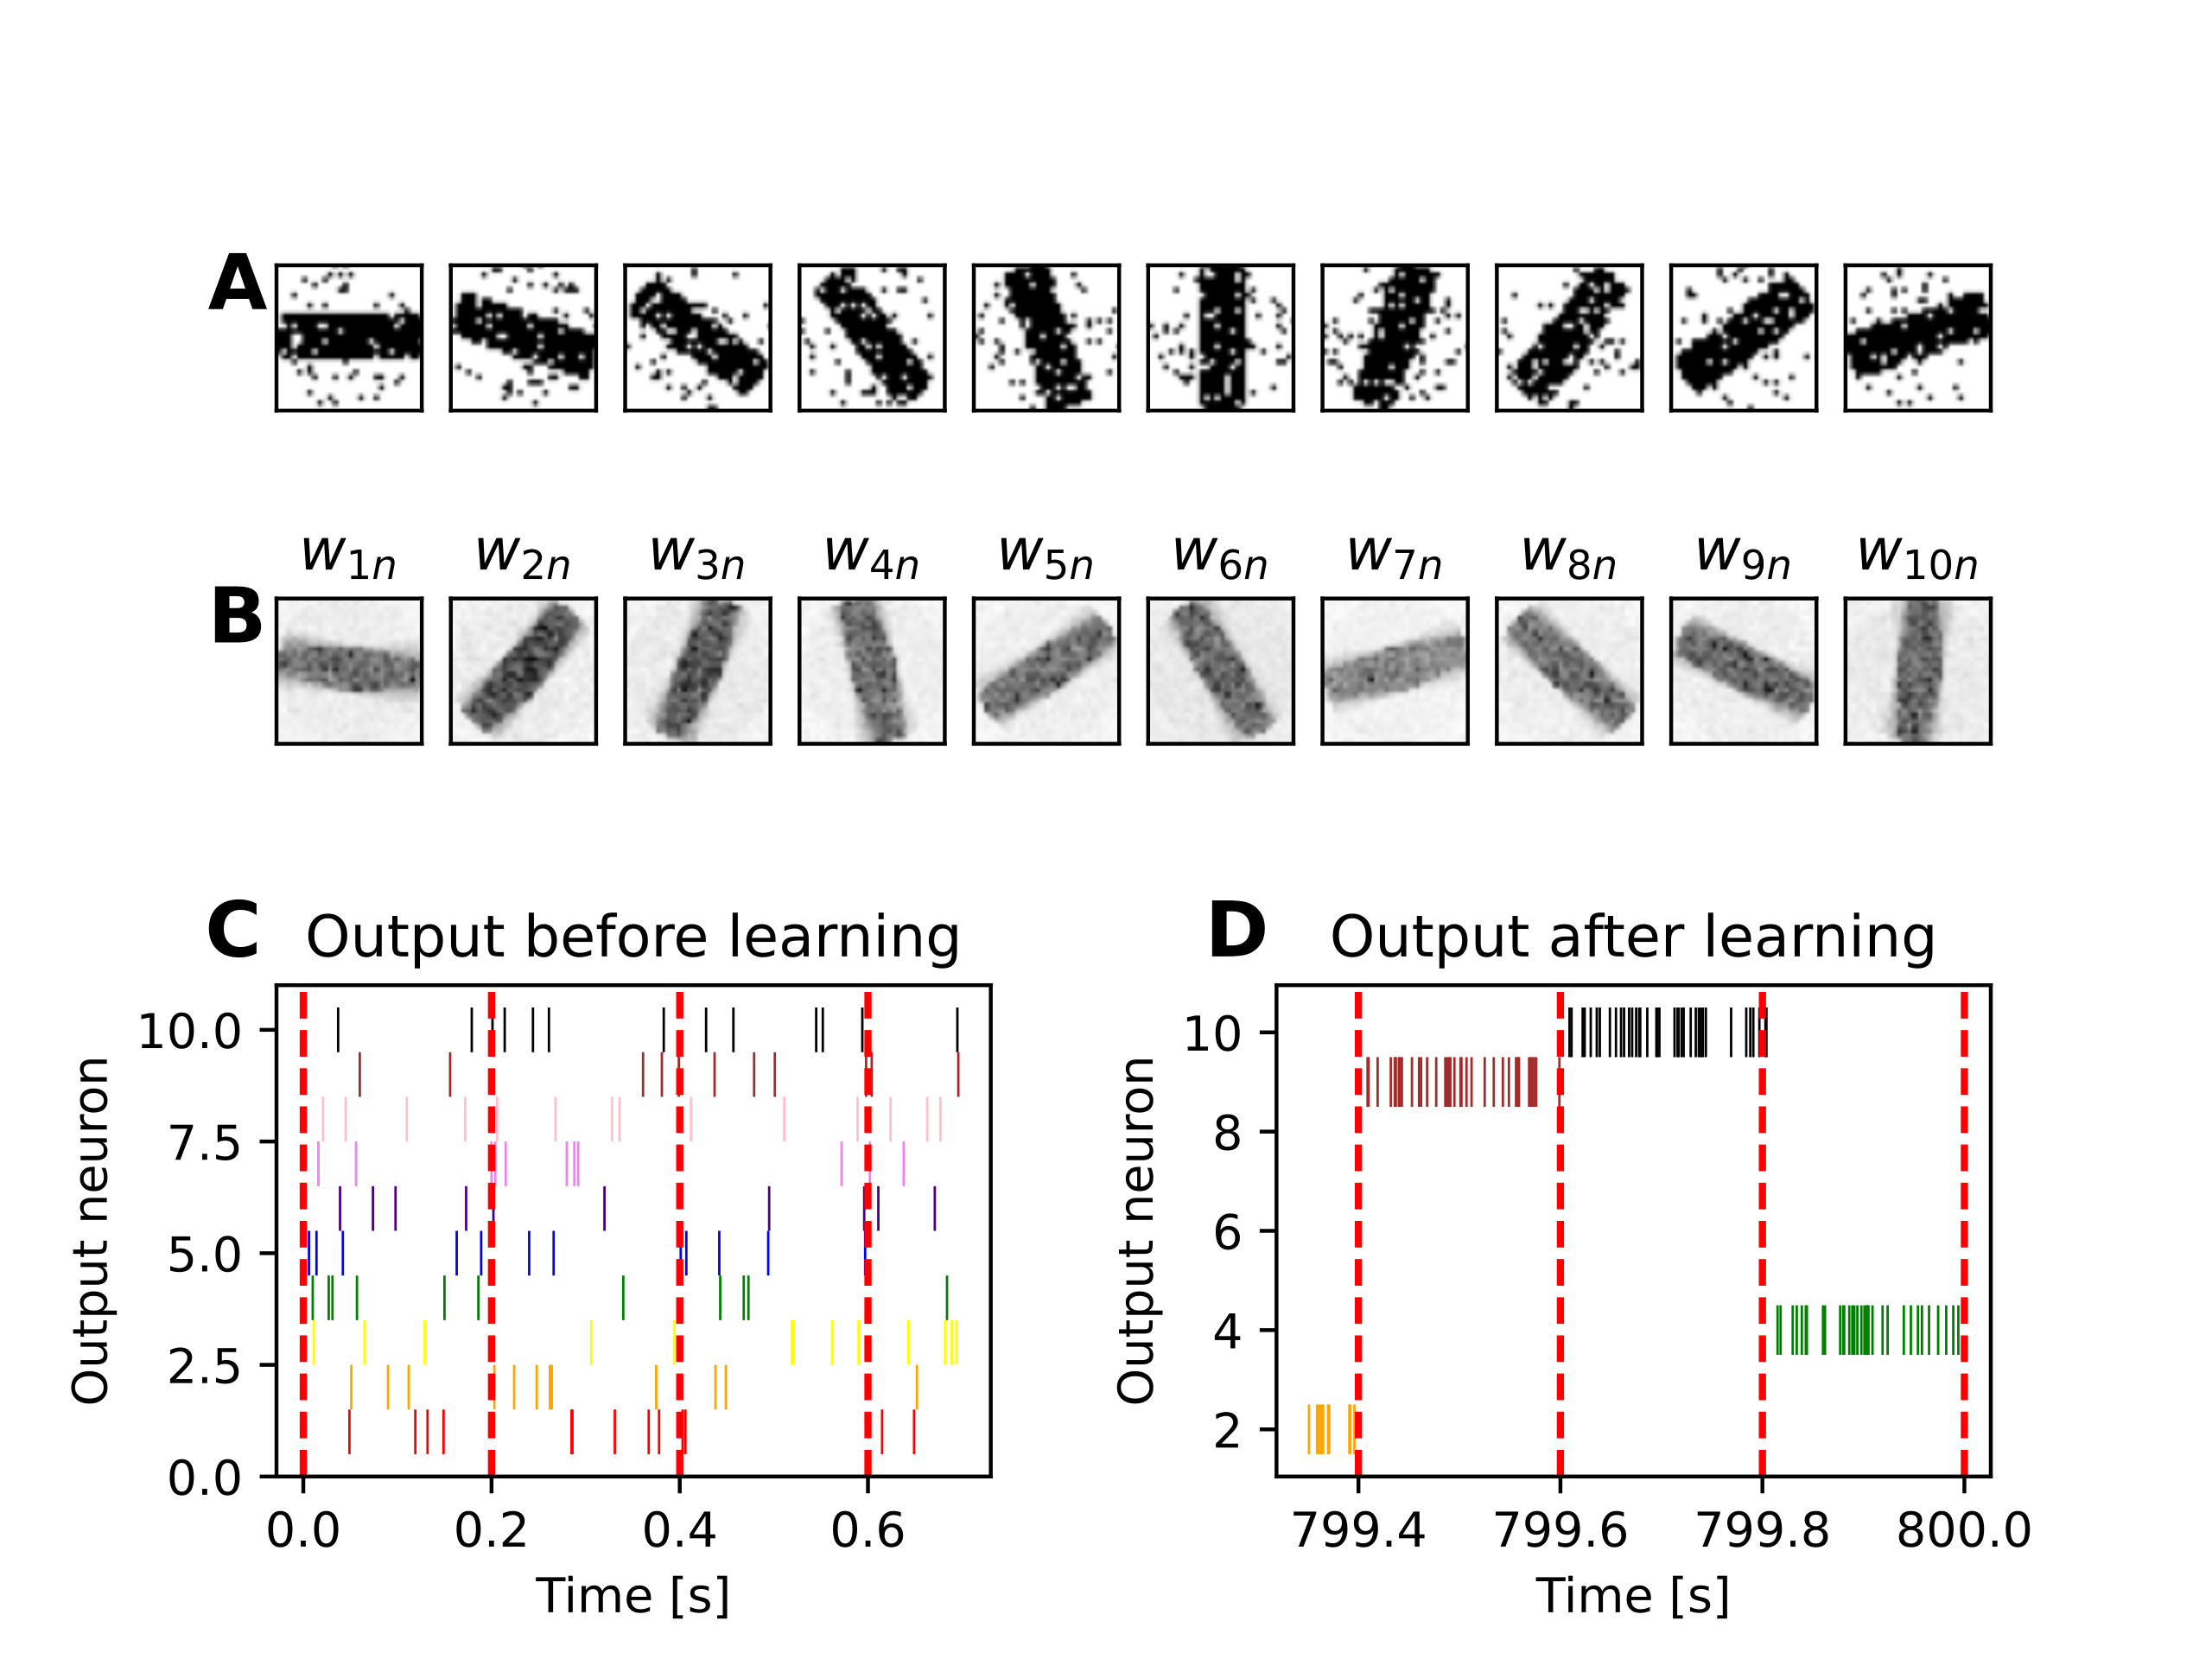
\includegraphics[width=\linewidth]{figures/angleAdaptiveInh/trainingPlot.png}
  \caption{\textbf{Training.} \textbf{A} Examples of 29 x 29-pixel input images of rotated bars and background noise. \textbf{B} Learned weights of the connections between input and output neurons. \textbf{C, D} Spike activity expressed by the output neurons before and after the training of the network. }
  \label{fig:angleNetworkAdaptiveInhibitionTraining}
\end{figure}

\begin{figure}
  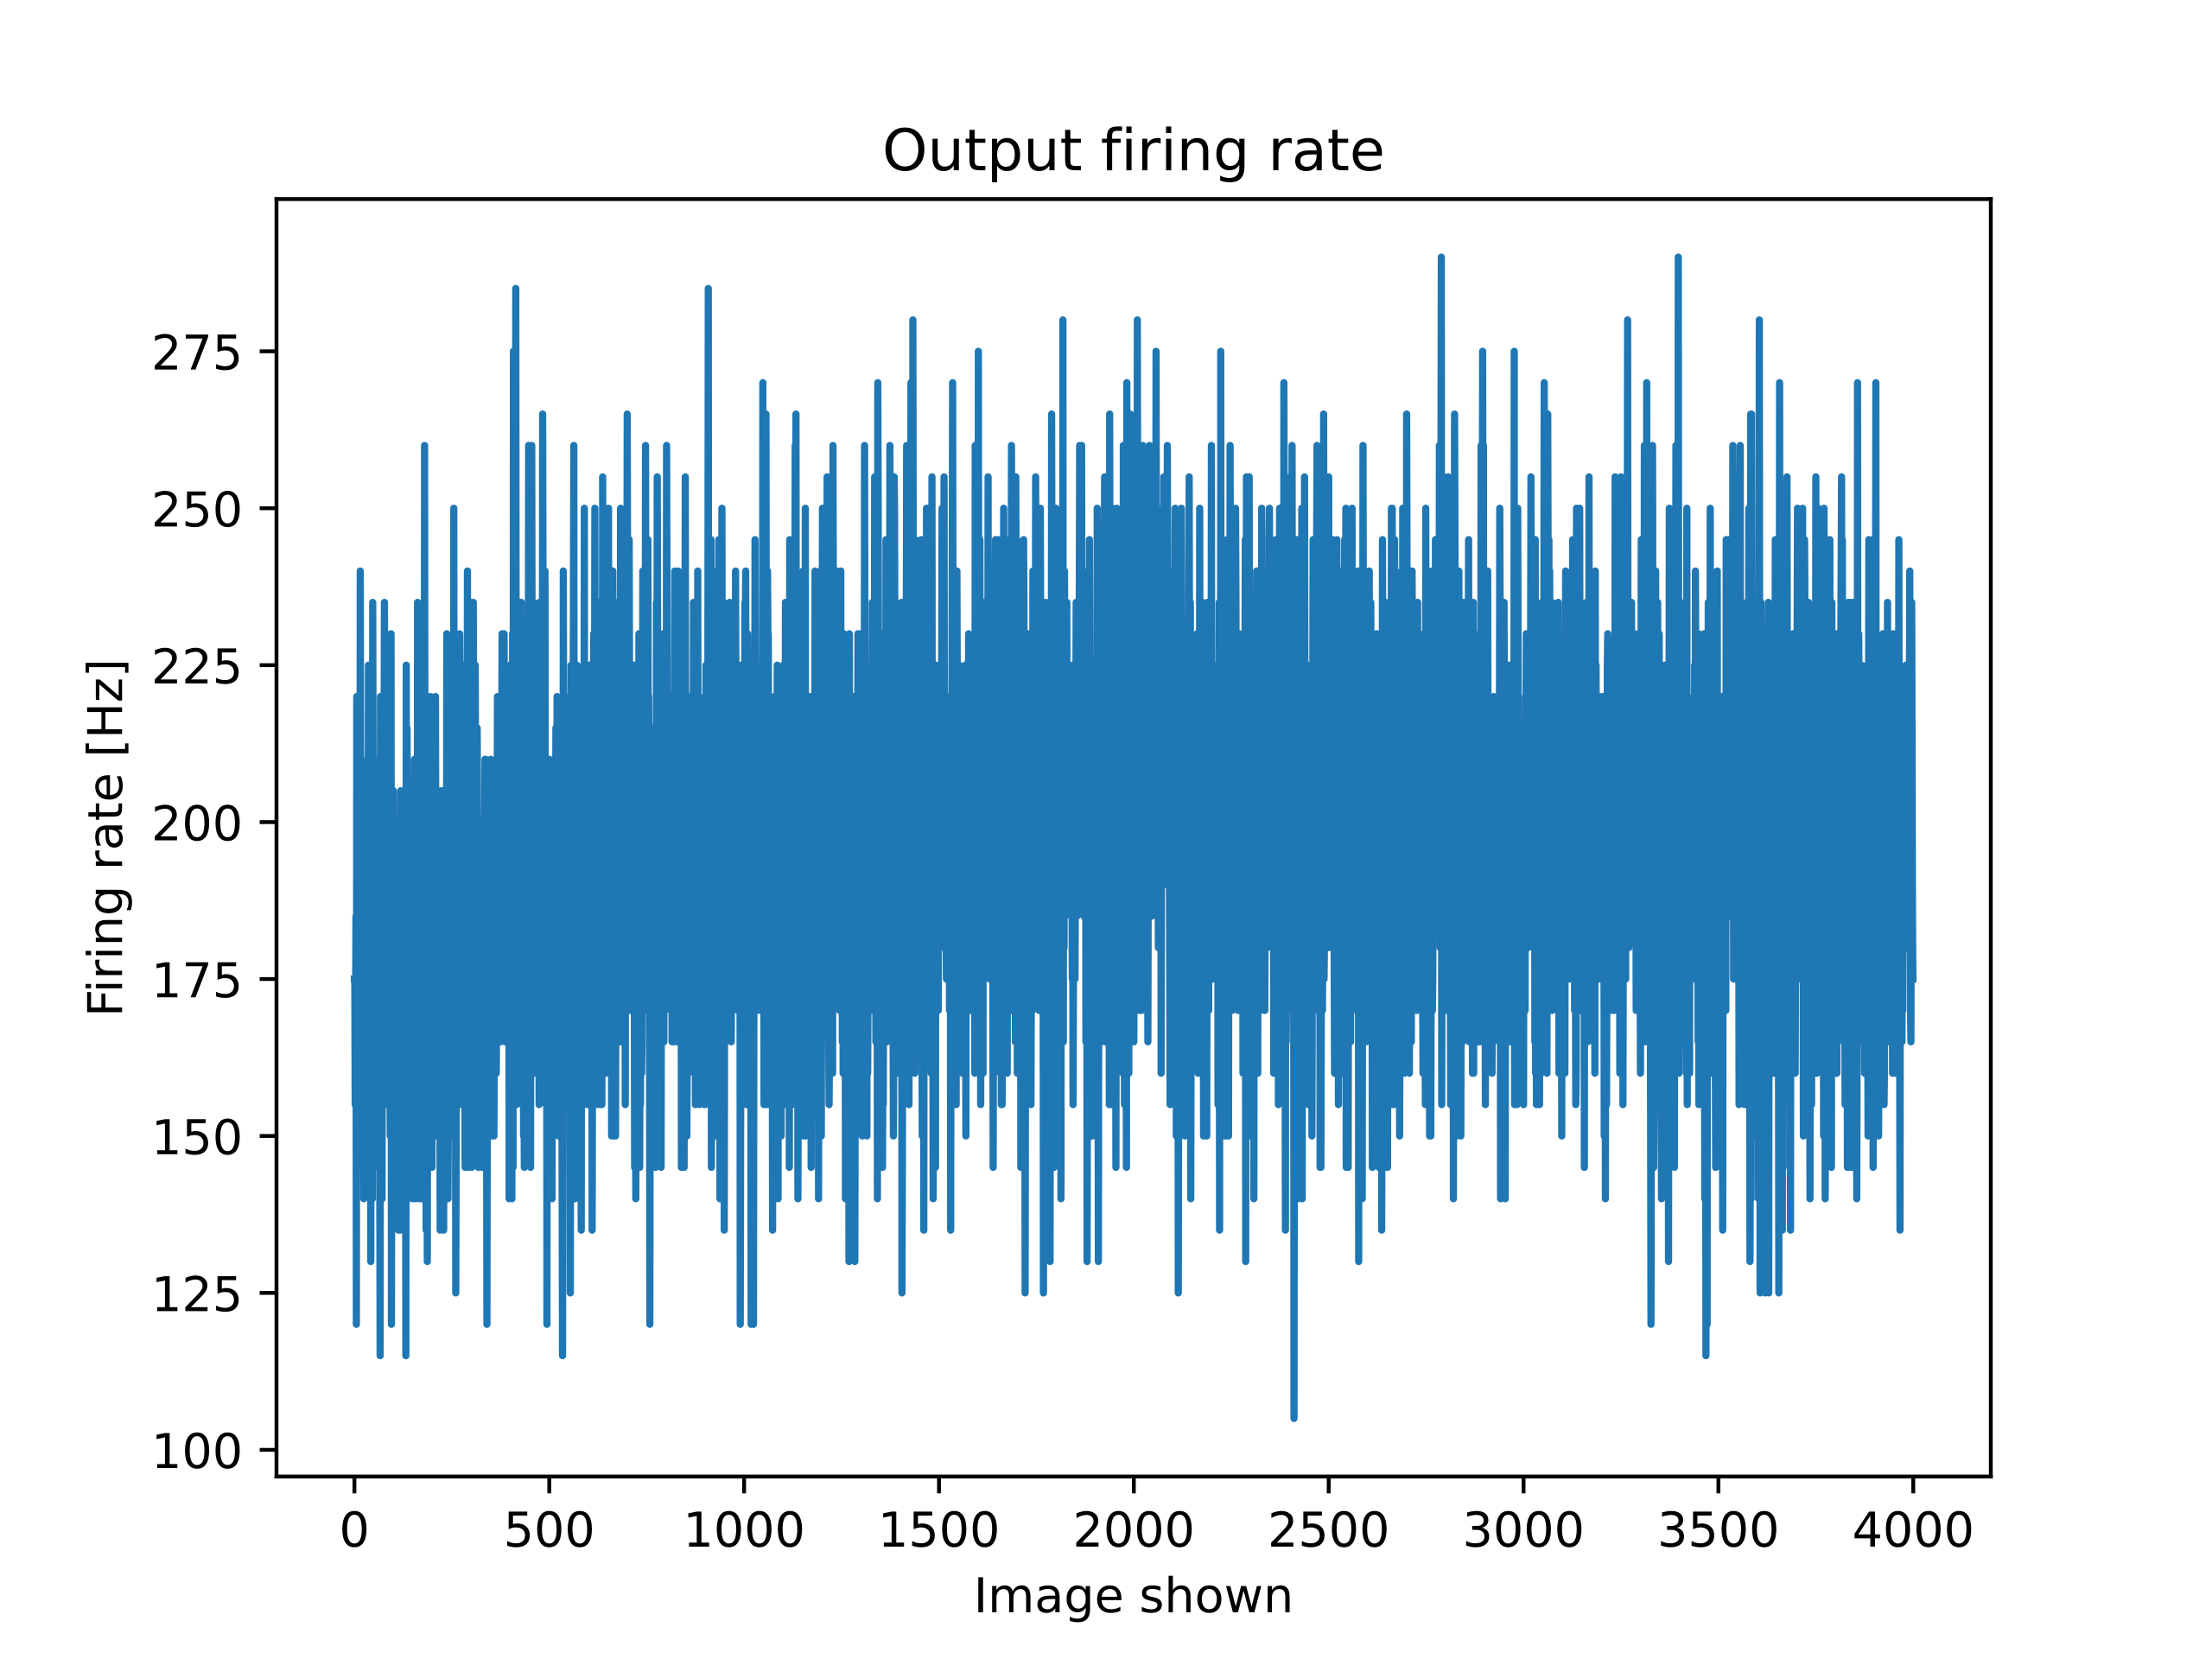
\includegraphics[width=\linewidth]{figures/angleAdaptiveInh/outputFiringRate.png}
  \caption{ Firing rate of all output neurons combined over the training process. }
  \label{fig:angleNetworkAdaptiveInhibitionOutputFiringRate}
\end{figure}

\begin{figure}
  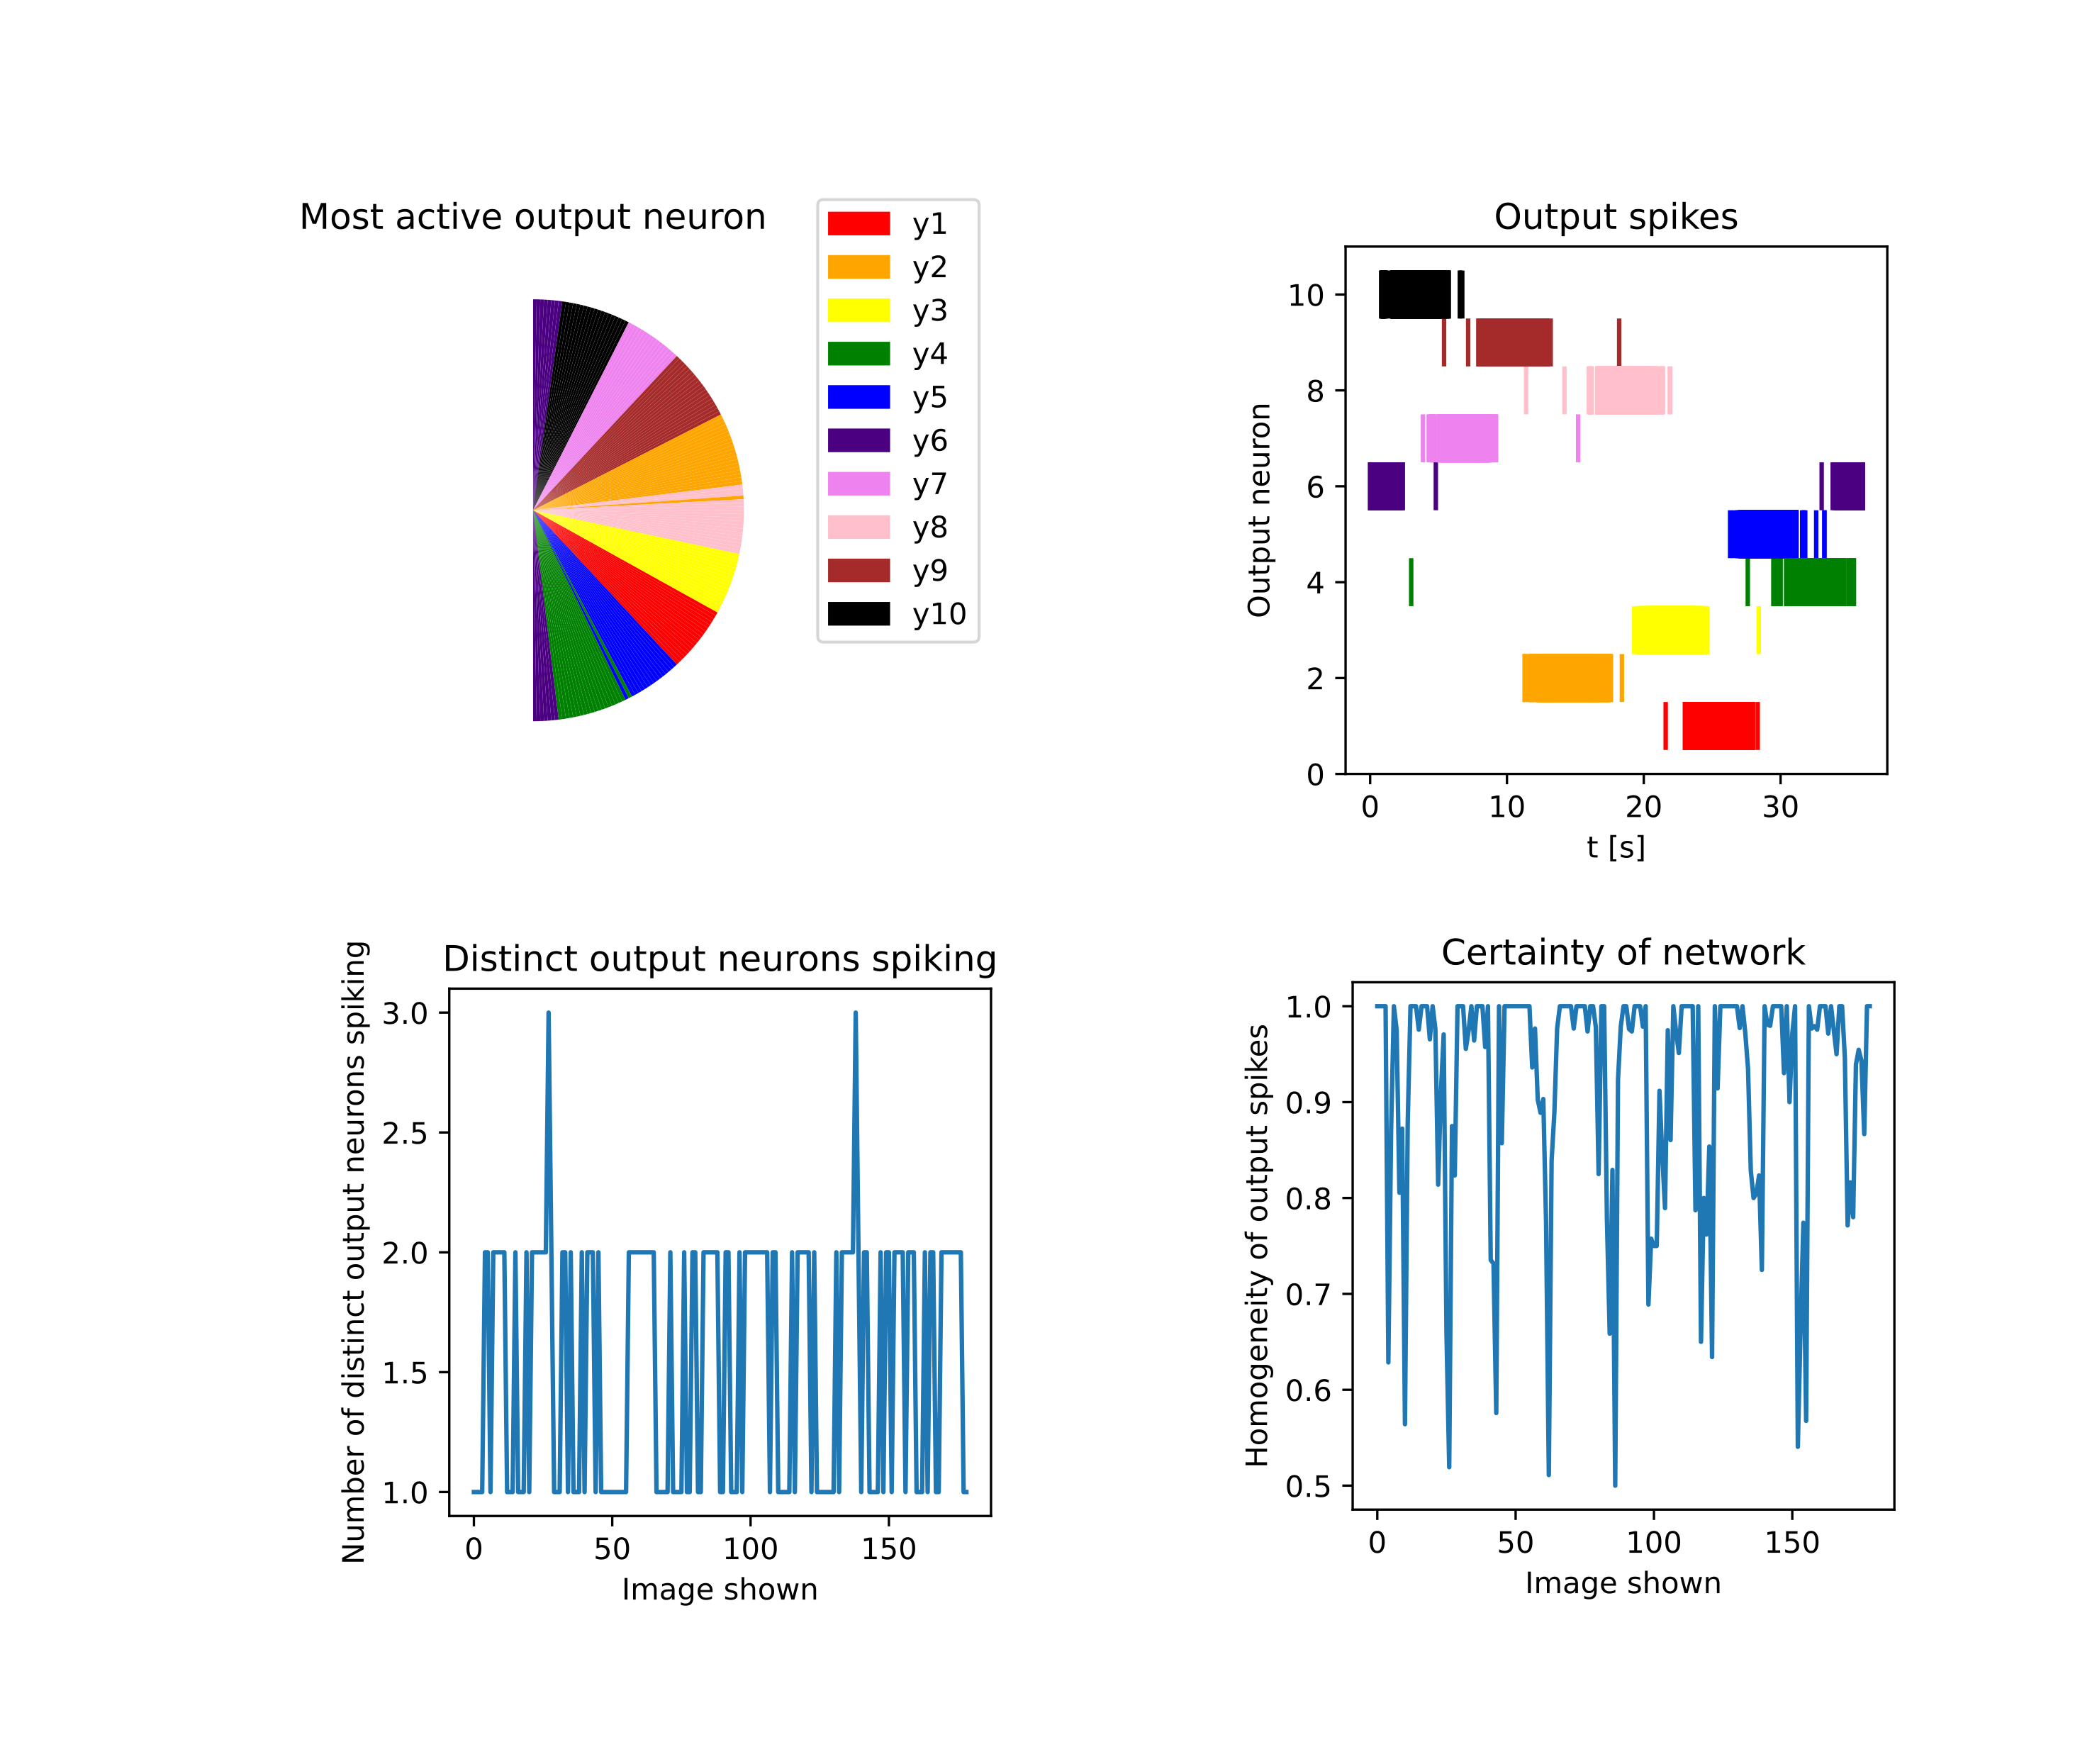
\includegraphics[width=\linewidth]{figures/angleAdaptiveInh/validation.png}
  \caption{\textbf{Validation.} \textbf{A} Most active output neuron depending on orientation of the training image. Training images were shown for 200 ms of each possible orientation in 1° steps. \textbf{B} Spike activity expressed by the output neurons during the validation process described in (\textbf{B}). \textbf{C} Number of distinct output neurons active during the presentation of each validation image. \textbf{D} Proportion (accuracy) of most active output neuron to activity of all other output neurons during the presentation duration of each training image.}
  \label{fig:angleNetworkAdaptiveInhibitionValidation}
\end{figure}